One of the most popular knowledge graphs is Freebase. Although the it is not maintained anymore since it was integrated into Wikidata~\cite{Tanon2016FromFT}, the benchmark datasets derived from it are still widely used. One of those benchmark datasets is the \emph{FB15k} dataset introduced by Bordes et al. in 2013~\cite{Bordes2013TranslatingEF}, whose name resembles the fact that it covers roughly \num{15000} Freebase entities. On its basis, Toutanova and Chen introduced the FB15k-237 in 2015~\cite{Toutanova2015ObservedVL}, whose purpose was to create a more meaningful benchmark by eliminating trivially predictable facts. For example, if FB15k-237 covers a relation like $(x, contains, y)$, it does not include its inverse relation $(y, part~of, x)$, because good performance resulting from such trivial, mutual predictions detracts from more interesting cases. In 2020, Safavi and Koutra were pushing further into this and published the CoDEx datasets, which are derived from FB15k-237 and two other datasets, that cover more diverse content and in turn pose a greater challenge than FB15k and FB15k-237~\cite{Safavi2020CoDExAC}. From the three provided datasets, CoDEx-S, CoDEx-M and CoDEx-L, the IRT splits by Hamann, on which this work is based, focuses on the CoDEx-M dataset. Table~\ref{tab:5_experiments/1_data_sources/1_knowledge_graphs/benchmark_datasets} gives an overview of the scales of FB15k, FB15k-237 and CoDEx-M. CoDEx-M actually contains additional negative facts that are excluded here as this work focuses on the common open-world scenario.

\begin{table}[h]
    \centering
    \begin{tabular}{| l | r | r | r | r | r |}
    \hline

    \multicolumn{1}{|c|}{\textbf{Dataset}} &
    \multicolumn{1}{|c|}{\textbf{#Entities}} &
    \multicolumn{1}{|c|}{\textbf{#Relations}} &
    \multicolumn{3}{|c|}{\textbf{#Facts}} \\

    \multicolumn{1}{|c|}{} &
    \multicolumn{1}{|c|}{} &
    \multicolumn{1}{|c|}{} &
    \multicolumn{1}{|c|}{\textbf{Train}} &
    \multicolumn{1}{|c|}{\textbf{Valid}} &
    \multicolumn{1}{|c|}{\textbf{Test}} \\

    \hline \hline

    FB15k     & \num{14951} & \num{1345} & \num{483142} & \num{50000} & \num{59071} \\
    FB15k-237 & \num{14541} & \num{237}  & \num{272115} & \num{17535} & \num{20466} \\
    CoDEx-M   & \num{17050} & \num{51}   & \num{185584} & \num{10310} & \num{10311} \\

    \hline
\end{tabular}

    \caption{Comparison of popular KGC benchmark datasets}
    \label{tab:5_experiments/1_data_sources/1_knowledge_graphs/benchmark_datasets}
\end{table}

As for the above KGC benchmark datasets, a graph's fact subset is usually further split into training, validation and test subsets. Thereby, the splits are created so that there are training, validation and test facts for possibly every entity. In contrast to that common approach, in his work on zero-shot learning, Hamann creates new splits from FB15k-237 and CoDEx-M that distinguish between so-called \emph{closed-world (CW) entities}, that are seen during training, and \emph{open-world (OW) entities}, which are not seen during training, to optimize prediction for unknown entities.

\begin{figure}
    \centering
    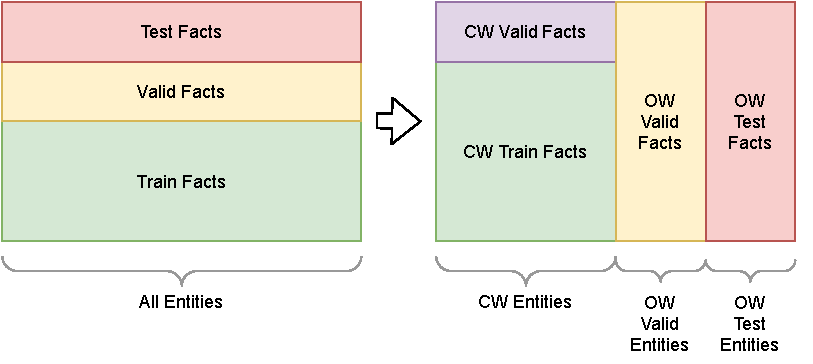
\includegraphics[width=\textwidth]{5_experiments/1_data_sources/1_knowledge_graphs/irt_split}
    \caption{Difference between (a) conventional and (b) the IRT fact splits - the IRT fact split focuses on open-world entities that must stay unseen during training - "CW" = "closed-world", "OW" = "open-world", "Ents" = "Entities"}
    \label{fig:5_experiments/1_data_sources/1_knowledge_graphs/irt_split}
\end{figure}

Figure~\ref{fig:5_experiments/1_data_sources/1_knowledge_graphs/irt_split} illustrates the difference the approach imposes on the fact split. The closed-world entities' facts are further split into closed-world training and closed-world validation facts to enable closed-world prediction in addition to open-world prediction. Closed-world training and closed-world validation facts only refer to closed-world entities, while at least one of an open-world facts' head or tail refers to an open-world entity. The open-world entities are properly divided into disjoint subsets of open-world validation and open-world test entities that do not appear in each other's fact sets. Table~\ref{tab:5_experiments/1_data_sources/1_knowledge_graphs/irt_splits} gives an overview of the dimensions of the entity and fact subsets.

\begin{table}[h]
    \centering
    \begin{tabular}{ l c r r r c r r c r r }
    \toprule
    
    \multicolumn{1}{l}{\textbf{Graph}} & \phantom &
    \multicolumn{1}{c}{\textbf{\thead{CW \\ Train \\ Ents}}} &
    \multicolumn{1}{c}{\textbf{\thead{CW \\ Train \\ Facts}}} &
    \multicolumn{1}{c}{\textbf{\thead{CW \\ Valid \\ Facts}}} & \phantom &
    \multicolumn{1}{c}{\textbf{\thead{OW \\ Valid \\ Ents}}} &
    \multicolumn{1}{c}{\textbf{\thead{OW \\ Valid \\ Facts}}} & \phantom &
    \multicolumn{1}{c}{\textbf{\thead{OW \\ Test \\ Ents}}} &
    \multicolumn{1}{c}{\textbf{\thead{OW \\ Test \\ Facts}}} \\

    \midrule

    FB15k-237 && \num{12057} & \num{214412} & \num{23778} && \num{1545} & \num{46503} && \num{816}  & \num{25423} \\
    CoDEx-M   && \num{11399} & \num{123650} & \num{13738} && \num{2918} & \num{41240} && \num{1896} & \num{27577} \\

    \bottomrule
\end{tabular}

    \caption{Dimensions of the IRT splits of the CoDEx-M and FB15K-237 datasets}
    \label{tab:5_experiments/1_data_sources/1_knowledge_graphs/irt_splits}
\end{table}
